\documentclass{standalone}

\usepackage{tikz}
\usetikzlibrary{shapes}
\usetikzlibrary{arrows}
\usetikzlibrary{calc,positioning}

\begin{document}
    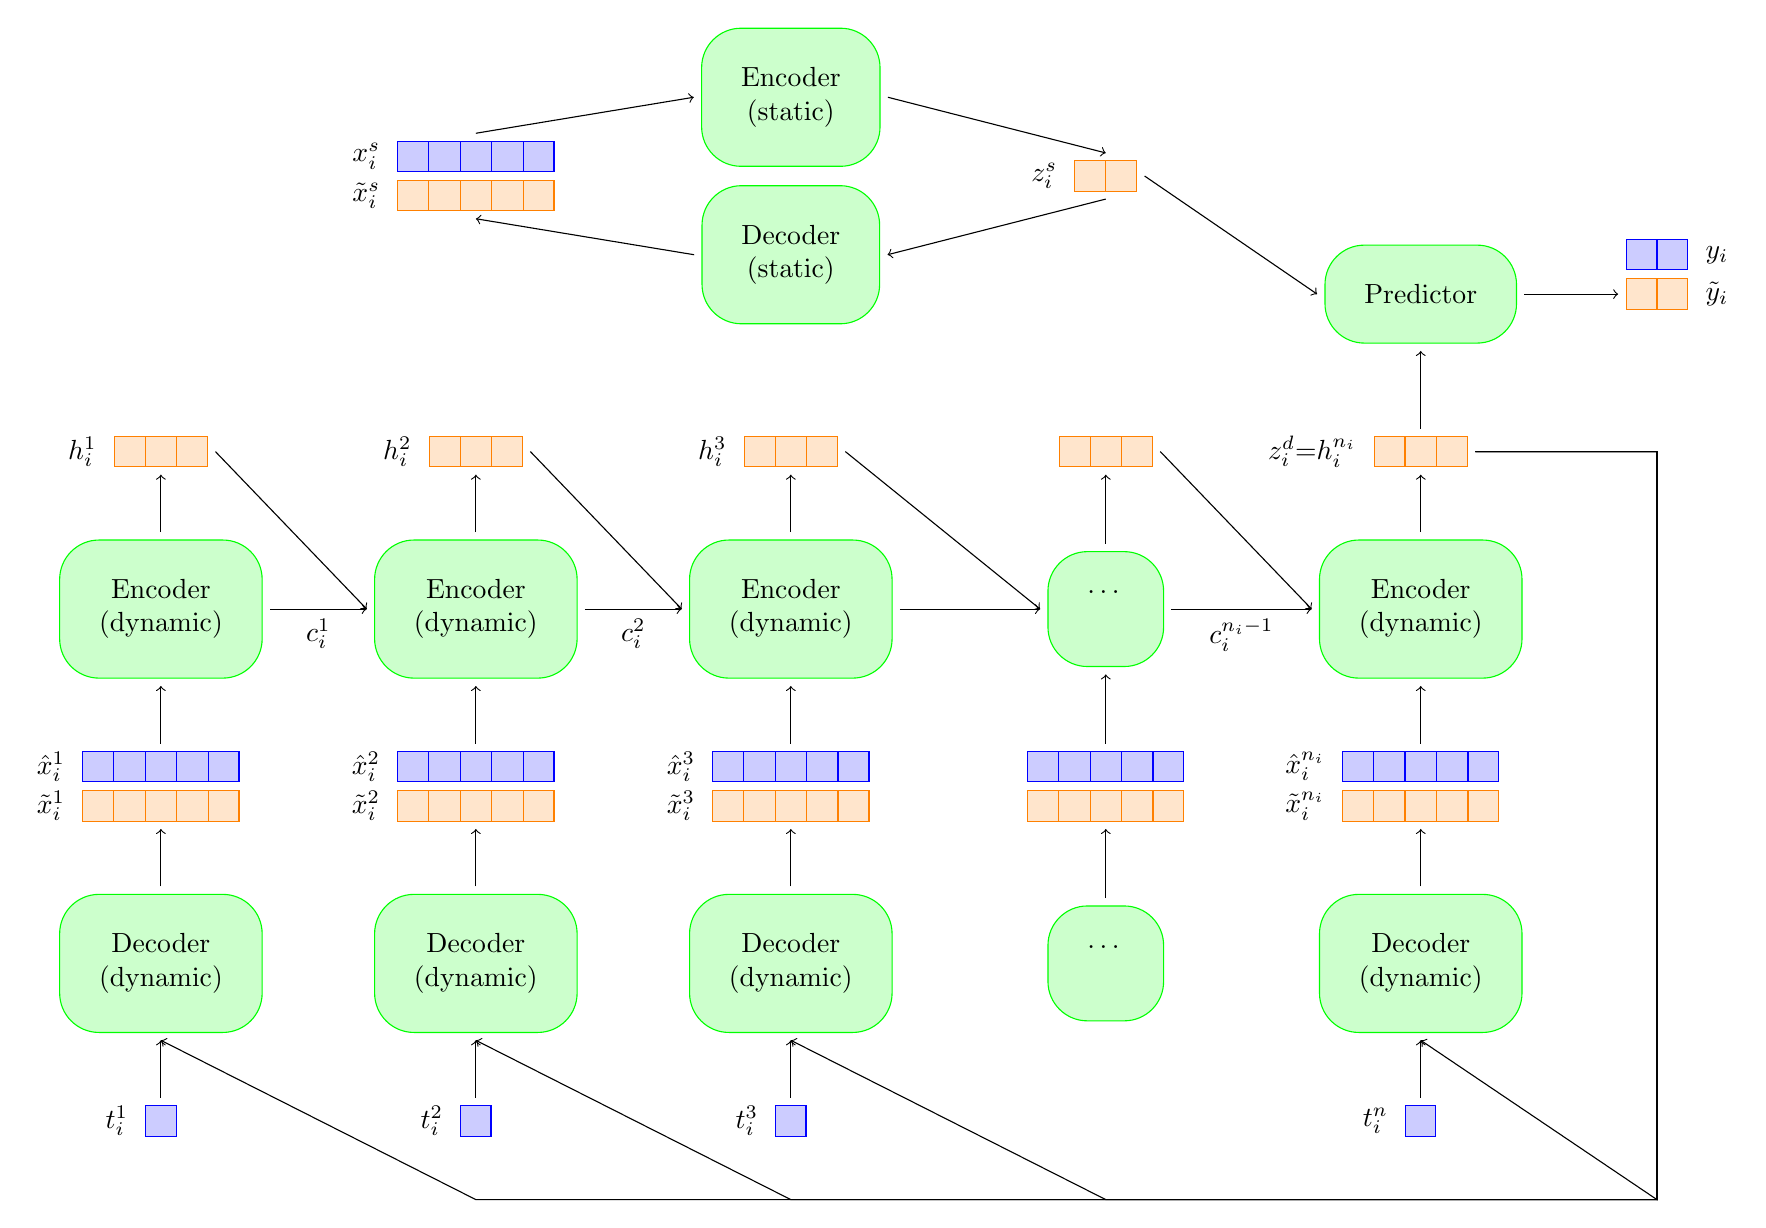
\begin{tikzpicture} [
        hid/.style 2 args={
            rectangle split,
            rectangle split horizontal,
            draw=#2,
            rectangle split parts=#1,
            fill=#2!20,
            outer sep=1mm},
        cell/.style={
            align=center,
            rectangle,
            rounded corners=5mm,
            draw=green,
            fill=green!20,
            inner sep=5mm,
            outer sep=1mm}]

    %draw first 3 columns 
    \foreach \step in {1,...,3} {
        \node[cell] (d\step) at (4*\step,0) {Decoder \\ (dynamic)};
        \node[hid={1}{blue},label=west:$t_i^\step$] (t\step) at (4*\step,-2) {};
        \draw[->] (t\step.north) -> (d\step.south);
        \node[hid={5}{orange},label=west:$\tilde{x}_i^\step$] (x_tilde\step) at
(4*\step,2){};
        \draw[->] (d\step.north) -> (x_tilde\step.south);
        \node[hid={5}{blue},label=west:$\hat{x}_i^\step$] (x_hat\step) at
(4*\step,2.5){};
        \node[cell] (e\step) at (4*\step,4.5) {Encoder \\ (dynamic)};
        \draw[->] (x_hat\step.north) -> (e\step.south);
        \node[hid={3}{orange},label=west:$h_i^\step$] (h\step) at (4*\step,6.5) {};
        \draw[->] (e\step.north) -> (h\step.south);
    }

    \foreach \step in {1,...,2} {
        \pgfmathtruncatemacro{\next}{add(\step,1)}
        \draw[->] (e\step.east) -> (e\next.west)
node[midway,below] {$c_i^\step$};
        \draw[->] (h\step.east) -> (e\next.west);
    }
    
    % draw the n_column 
    \node[cell] (d_n) at (20,0) {Decoder \\ (dynamic)};
    \node[hid={1}{blue},label=west:$t_i^n$] (t_n) at (20,-2) {};
    \draw[->] (t_n.north) -> (d_n.south);
    \node[hid={5}{orange},label=west:$\tilde{x}_i^{n_i}$] (x_tilde_n) at (20,2){};
    \draw[->] (d_n.north) -> (x_tilde_n.south);
    \node[hid={5}{blue},label=west:$\hat{x}_i^{n_i}$] (x_hat_n) at (20,2.5){};
    \node[cell] (e_n) at (20,4.5) {Encoder \\ (dynamic)};
    \draw[->] (x_hat_n.north) -> (e_n.south);
    \node[hid={3}{orange},label=west:$z_i^d {=} h_i^{n_i}$] (h_n) at (20,6.5) {};
    \draw[->] (e_n.north) -> (h_n.south);
    
    % draw the '...' column
    \node[cell] (e_dot) at (16,4.5) {\ldots\\};
    \node[cell] (d_dot) at (16,0) {\ldots\\};
    \node[hid={5}{orange}] (x_tilde_dot) at (16,2){};
    \draw[->] (d_dot.north) -> (x_tilde_dot.south);
    \node[hid={5}{blue}] (x_hat_dot) at (16,2.5){};
    \draw[->] (x_hat_dot.north) -> (e_dot.south);
    \node[hid={3}{orange}] (h_dot) at (16,6.5) {};
    \draw[->] (e_dot.north) -> (h_dot.south);

    % connect dots and columns
    \draw[->] (h3.east) -> (e_dot.west);
    \draw[->] (e3.east) -> (e_dot.west);
    \draw[->] (e_dot.east) -> (e_n.west) node[midway,below] {$c_i^{n_i-1}$};
    \draw[->] (h_dot.east) -> (e_n.west);
   
    % top layer
    \node[cell] (p) at (20,8.5) {Predictor};
    \node[hid={2}{orange},label=east:$\tilde{y}_i$] (y_tilde_i) at (23,8.5){};
    \node[hid={2}{blue},label=east:$y_i$] (y_i) at (23,9){};
    \draw[->] (p) -> (y_tilde_i);
    \draw[->] (h_n.north) -> (p.south);

    \foreach \step in {1,...,3} {
        \pgfmathtruncatemacro{\next}{add(\step,1)}
        \draw[->] (h_n.east) -- (23,6.5) -- (23,-3) -- (4*\next,-3) --
(d\step.south);
    }
    \draw[->] (h_n.east) -- (23,6.5) -- (23,-3) -- (d_n.south);
    \node[hid={2}{orange},label=west:$z_i^s$] (z_s) at (16,10){};
    \node[cell] (d_s) at (12,9) {Decoder \\ (static)};
    \node[cell] (e_s) at (12,11) {Encoder \\ (static)};
    \draw[->] (z_s.east) -> (p.west);
    \draw[->] (e_s.east) -> (z_s.north);
    \draw[->] (z_s.south) -> (d_s.east);
    \node[hid={5}{blue},label=west:$x_i^s$] (x_s) at (8,10.25){};
    \node[hid={5}{orange},label=west:$\tilde{x}_i^s$] (x_tilde_s) at (8,9.75){};
    \draw[->] (d_s.west) -> (x_tilde_s.south){};
    \draw[->] (x_s.north) -> (e_s.west){};
    
    \end{tikzpicture}
\end{document}
